\section{Evaluation}\label{sec:evaluation}
\subsection{Experimental Setup and Metrics}\label{sec:setup}
Microbenchmarks examine the scalability of independent synchronous updates; a macrobenchmark tests mixed file operations; applications measure transaction and persistent-publish completion rates.
Mechanism and cost analysis examines changes on synchronization paths, while recovery experiments check commit semantics.
We evaluate the GOOD12.1 implementation of Z-ParaPack.
The fio, FileMicro, and NATS comparisons include F2FS, XFS, Btrfs, ScaleLFS, and Z-LFS.
SQLite and extended Varmail compare against F2FS, Btrfs, ScaleLFS, Z-LFS, DeLFS, MAX, and F2FSJ; OceanBase includes all nine systems.

\begin{table}[t]\centering
\caption{Platform and system configuration.}\label{tab:platform}
\small\setlength{\tabcolsep}{3pt}
\begin{tabularx}{\columnwidth}{@{}P{.19\columnwidth}Y@{}}\toprule
Item & Configuration \\
\midrule
Host & Two Xeon Gold 5218 processors; 32 physical cores, 64 logical CPUs; Linux 7.2.9 \\
Storage & AF3UP44ZTEIG8T0A ZNS SSD; firmware OI1T1129; common 546-zone data region; active/open limits of sixteen each \\
Z-ParaPack & GOOD12.1; fifteen file-update lanes, one maintenance lane; sixteen owners and sixteen SIT shards \\
Native baselines & F2FS, XFS, Btrfs \\
Research baselines & ScaleLFS and Z-LFS: same-kernel ports; DeLFS: local adaptation; MAX and F2FSJ: prototype deployments \\
\bottomrule\end{tabularx}
\end{table}

All systems use the common ZNS region in Table~\ref{tab:platform}.
Z-ParaPack, F2FS, and ScaleLFS place fixed metadata in a 24\,GiB region on a conventional device, with main DATA/NODE on ZNS.
XFS uses a 32\,GiB conventional metadata region and ZNS realtime file data, with \texttt{max\_open\_zones=8}.
Btrfs and Z-LFS use a single ZNS layout.
fio uses logical CPUs 0 through 63.
SQLite clients bind to even-numbered CPUs, with Z-ParaPack owners on non-uniform memory access (NUMA) node~0; other Filebench and application workloads use the default owner configuration.

Z-ParaPack retains ordinary DATA/NODE writes, FLUSH, and the FUA that terminals require.
We use fio 3.28, Filebench 1.4.9.1, NATS Server 2.15.0, and nats.go 1.45.0.
Initialization and preloading precede timing; performance runs disable probes, while allocation counts and path diagnostics use separate runs.
Application baselines include observations across dates under the same implementation, configuration, and workload recipe; comparisons use descriptive statistics.
Table~\ref{tab:workloads} defines operations and completion metrics.
Each result specifies run counts and aggregation.
Asterisks in figures identify local adaptations or ports; daggers identify prototype deployments.
Supplementary Sections~S1 and S2 retain complete Filebench and application results and SQLite latency distributions.

\begin{table}[t]\centering
\caption{Benchmark operations, synchronization semantics, and completion metrics.}\label{tab:workloads}
\small\setlength{\tabcolsep}{3pt}
\begin{tabularx}{\columnwidth}{@{}P{.19\columnwidth}Y@{}}\toprule
Workload & Operations, synchronization, and metric \\
\midrule
FileMicro & Sixteen independent 1\,GiB files; 2\,KiB random writes; WriteRandDsync maps dsync to O\_SYNC. Metric: successful synchronous writes/s. \\
Varmail & One process, sixteen threads; deletes, creates, reads, random appends, and two explicit fsync operations~\cite{r10}. Metric: total flowops/s, including non-write operations. \\
NATS JetStream & Native FileStorage; sixteen streams and publishing connections; \texttt{sync\_interval=always}~\cite{r11}. Metric: successful publishes per second, from a common barrier through the final acknowledgment (ACK). \\
SQLite & Eight databases/64\,KiB or sixteen databases/16\,KiB; each worker updates an independent database, one row per transaction; write-ahead logging (WAL), \texttt{synchronous=FULL}, 1000-page automatic checkpoint threshold. Metrics: transactions/s over the full interval including connection closure; transaction latency. \\
\bottomrule\end{tabularx}
\end{table}

PACK admission checks the inode's dirty DATA page count at synchronization entry.
The limit is sixteen pages for ordinary fio conditions and 1024 pages for 128\,KiB updates and path diagnostics.
Filebench and application benchmarks set the limit to zero, removing this count limit while retaining closure and resource feasibility checks.
Requests exceeding the limit fall back to the original synchronization path.
Reproduction materials retain complete formatting, mount, module-version, and workload recipes.

\subsection{Microbenchmarks: Concurrent Synchronous Updates}\label{sec:micro}
Z-ParaPack's advantage emerges as independent file-update concurrency increases.
fio uses \texttt{psync}, \texttt{pthread}, \texttt{iodepth=1}, and \texttt{direct=0}.
Each thread updates its own file and waits for \texttt{fsync} after every write.
Files total 16\,GiB; timing lasts 600 seconds after prefill and synchronization.
Figure~\ref{fig:scaling}(a, b) covers one through 32 threads with 4\,KiB and 64\,KiB updates, corresponding to one and sixteen DATA pages.
Completion rates include durability of DATA and related NODEs.
Each of the sixteen synchronous-random-write conditions has one run.

\begin{figure*}[t]\centering
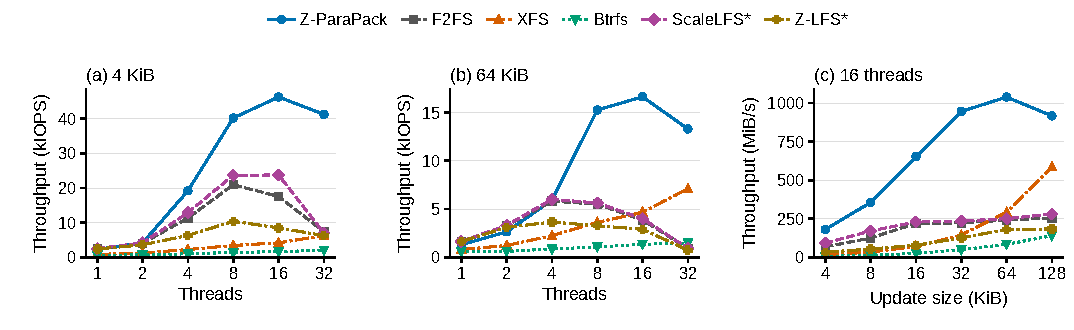
\includegraphics[width=\textwidth]{./figures/compact_fio_scalability.pdf}
\caption{Synchronous random overwrites. (a, b) Concurrency scaling with 4\,KiB and 64\,KiB updates; (c) update-size comparison at sixteen threads.}\label{fig:scaling}
\end{figure*}

At 32 threads, Z-ParaPack reaches 41.27\,kIOPS for 4\,KiB updates, 5.58$\times$ F2FS (7.40\,kIOPS), the fastest baseline under that condition.
For 64\,KiB updates, it reaches 13.30\,kIOPS, 1.87$\times$ the fastest baseline, XFS (7.12\,kIOPS).

Among the concurrency points in Figure~\ref{fig:scaling}, Z-ParaPack exceeds the fastest corresponding baseline from four threads for 4\,KiB and eight threads for 64\,KiB.
At eight threads, 64\,KiB updates already reach 15.26\,kIOPS, 2.71$\times$ the fastest baseline, ScaleLFS.
Thirty-two workers reuse fifteen file-update lanes within the same zone region and active/open limits.
Request count can exceed lane count because completed PACKs return append permission for subsequent updates.

At sixteen threads, Z-ParaPack achieves the highest completed bandwidth for every tested update size: 4, 8, 16, 32, 64, and 128\,KiB.
Its bandwidth reaches 1.56$\times$ to 4.02$\times$ the fastest baseline under each condition.
Figure~\ref{fig:scaling}(c) retains synchronization after every write, covering single-page through 128\,KiB multipage updates.

FileMicro exercises the same problem through O\_SYNC writes.
Sixteen threads issue 2\,KiB synchronous random writes to independent files, with one write operation per WriteRandDsync worker.
Z-ParaPack reaches 1.91$\times$ the successful-write rate of ScaleLFS, the fastest baseline (Figure~\ref{fig:filemicro}).
The comparison runs for 300 seconds, with one independent run per system across six systems.
Bars show run rates.

\begin{figure}[t]\centering
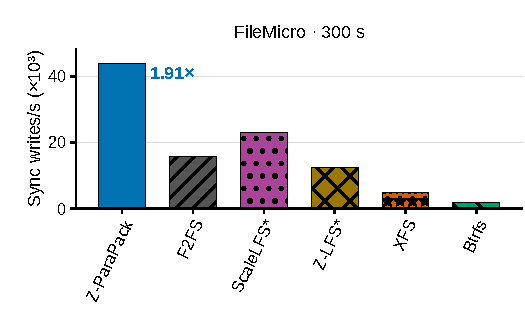
\includegraphics[width=\columnwidth]{./figures/main_filemicro_throughput.pdf}
\caption{FileMicro synchronous random writes. The blue ratio compares against the fastest baseline.}\label{fig:filemicro}
\end{figure}

\subsection{Macrobenchmark: Mixed File Operations}\label{sec:macro}
Extended Varmail combines deletes, creates, reads, appends, and explicit \texttt{fsync} calls into a file-operation stream~\cite{r10}.
Z-ParaPack reaches 101,538.68\,flowops/s, 33.7\% above the fastest baseline, ScaleLFS at 75,955.69\,flowops/s (Figure~\ref{fig:varmail}).
The workload uses 10,000 files, a mean file size of 1\,MiB, mean appends of about 64\,KiB, and a 128\,KiB append upper bound.
Total flowops include non-write operations and measure completed mixed operations.

\begin{figure}[t]\centering
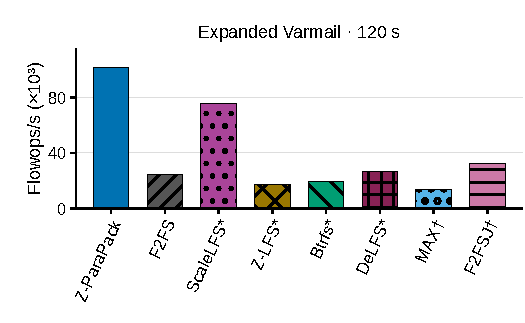
\includegraphics[width=\columnwidth]{./figures/main_varmail_extended.pdf}
\caption{Extended Varmail total flowops/s, including non-write operations. Bars show geometric means of run rates. Asterisks identify local adaptations; daggers identify prototypes.}\label{fig:varmail}
\end{figure}

All eight systems run for 120 seconds.
DeLFS, MAX, and F2FSJ each have two runs; the others each have three.
The mixed workload alternates creation, deletion, and synchronization, extending the single-operation write comparison to filesystem workflows that include namespace changes.

\subsection{Applications: Database Transactions and Persistent Services}\label{sec:applications}
SQLite, NATS, and OceanBase count completed transactions, persistent-publish ACKs, and completed event transactions, respectively.
Controlled clients drive these database and messaging systems to test whether parallel filesystem commits improve application completion rates.

\textbf{SQLite transactions and extreme tail latency.}
Each SQLite worker updates an independent database, modifying one row per transaction.
Table~\ref{tab:workloads} specifies WAL, \texttt{synchronous=FULL}, and automatic checkpoints.
The sixteen-database/16\,KiB configuration reaches 1.94$\times$ its fastest baseline, F2FS; eight databases/64\,KiB reaches 1.37$\times$ its fastest baseline, ScaleLFS (Figure~\ref{fig:sqlite-rate}).
Both configurations run for 120 seconds.
Every system has three runs with sixteen databases.
With eight databases, DeLFS, MAX, and F2FSJ have two runs each, and the others have three.
Bars show geometric means of independent run rates.

\begin{figure}[t]\centering
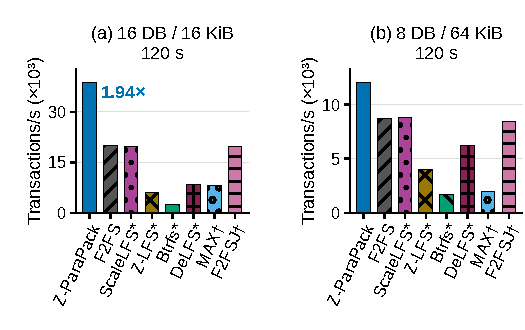
\includegraphics[width=\columnwidth]{./figures/main_sqlite_throughput.pdf}
\caption{SQLite transaction completion rates. (a, b) Sixteen databases/16\,KiB and eight databases/64\,KiB. Blue ratios compare against the fastest baseline in each configuration. Bars show geometric means. Asterisks identify local adaptations; daggers identify prototypes.}\label{fig:sqlite-rate}
\end{figure}

Higher throughput accompanies lower p99.9.
Z-ParaPack achieves the lowest p99.9 among all eight systems in both configurations.
With sixteen databases/16\,KiB, its 13.89\,ms is 73.4\% below Btrfs at 52.14\,ms, the lowest-latency baseline.
With eight databases/64\,KiB, its 10.75\,ms is 23.1\% below ScaleLFS at 13.99\,ms, the lowest-latency baseline.
Throughput and p99.9 comparisons use the fastest and lowest-latency baseline, respectively, within each configuration.

\begin{figure}[t]\centering
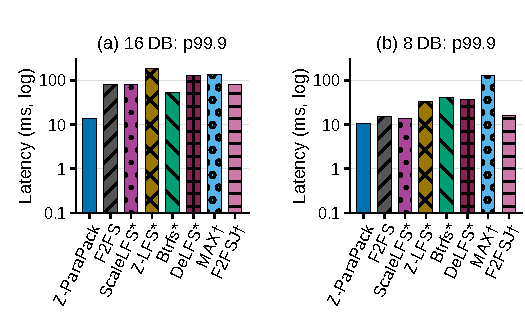
\includegraphics[width=\columnwidth]{./figures/main_sqlite_p999.pdf}
\caption{SQLite p99.9 with (a) sixteen databases/16\,KiB and (b) eight databases/64\,KiB. Millisecond axes use logarithmic scales with a 0.1\,ms bar baseline. Bars show geometric means of run-level quantiles. Asterisks identify local adaptations; daggers identify prototypes.}\label{fig:sqlite-tail}
\end{figure}

Transaction latency includes transaction start, update, commit, and lock-conflict retries before success.
For each run, we merge worker histograms in integer microseconds and compute nearest-rank p99.9.
We then take the geometric mean of these run-level quantiles.
Transaction rates cover the complete run interval, including connection closure.

\textbf{NATS persistent publishing.}
NATS JetStream publishes persistently across sixteen streams.
Z-ParaPack reaches 1.88$\times$ the successful-publish rate of ScaleLFS, the fastest baseline (Figure~\ref{fig:nats}).
Messages contain JSON from real AWS CloudWatch records~\cite{r12}, with sixteen fixed publishing connections and native FileStorage using \texttt{sync\_interval=always}~\cite{r11}.
Completion rates span the common publishing barrier through the final ACK, including waits for persistence confirmation.
The comparison lasts 300 seconds, with one independent run per system across six systems.

\begin{figure}[t]\centering
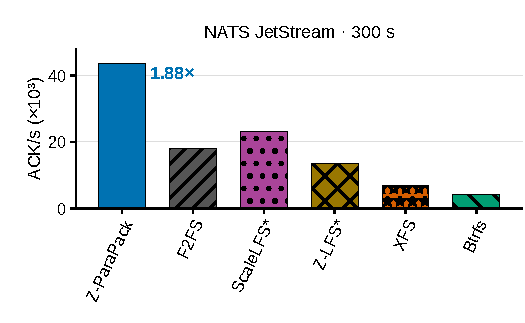
\includegraphics[width=\columnwidth]{./figures/main_nats_throughput.pdf}
\caption{NATS JetStream successful-publish rates. The blue ratio compares against the fastest baseline.}\label{fig:nats}
\end{figure}

\textbf{OceanBase multi-tenant event commits.}
With 128 OceanBase clients, Z-ParaPack increases mean throughput by 69.6\% over F2FS controls from the same cohort.
Throughput exceeds ScaleLFS and DeLFS by 66.0\% and 38.7\%, respectively.
Figure~\ref{fig:oceanbase} reports absolute event completion rates for all nine systems.

The workload uses two colocated, independent, single-replica OceanBase instances, with sixteen tenants and 128 closed-loop clients in total.
It preserves order within each repository while replaying 865,942 issue and pull-request events from the complete UTC day of January 6, 2025, in GH Archive~\cite{r15}.
Each event executes one autocommit transaction that retains the full JSON and reconstructs the entity's latest state.
The instances together use 32 logical service CPUs and 96\,GiB of configured memory; the database handles underlying log synchronization.

Completion rate divides all input events by wall-clock time from common client release until all clients exit.
Each baseline has two independent fresh-filesystem runs.
Comparisons use the corresponding cohort's GOOD controls and arithmetic means of run-level metrics; the GOOD bar pools eight observations.
Supplementary Section~S3 retains complete cohort results, latency distributions, and protocols.

\begin{figure}[t]\centering
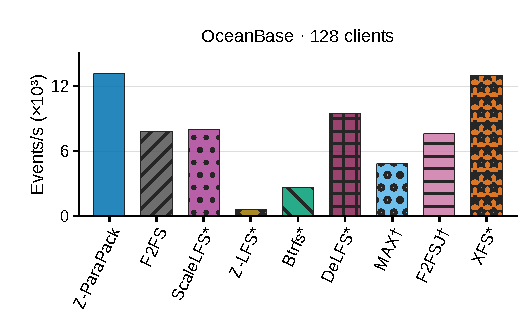
\includegraphics[width=\columnwidth]{./figures/main_oceanbase_throughput.pdf}
\caption{OceanBase full-JSON event completion rates. Bars show arithmetic means. Z-ParaPack pools eight observations, with two per baseline; text comparisons use matching cohort controls. Asterisks identify local adaptations; daggers identify prototypes.}\label{fig:oceanbase}
\end{figure}

\subsection{Mechanisms and Costs}\label{sec:cost}
\textbf{Shared-allocation intervals.}
F2FS shared-allocation intervals grow with concurrency; Z-ParaPack separates independent updates' append state across lanes.
In the request-correlated diagnostics of Figure~\ref{fig:breakdown}, increasing threads from eight to 32 raises F2FS combined DATA/NODE curseg time from 1.197 to 38.369\,ms.
The full sampled \texttt{fsync} grows from 2.716 to 40.845\,ms.
At eight, sixteen, and 32 threads, Z-ParaPack combined curseg time stays below 0.18\,ms, and the full sampled call stays below 1.4\,ms.

\begin{figure*}[t]\centering
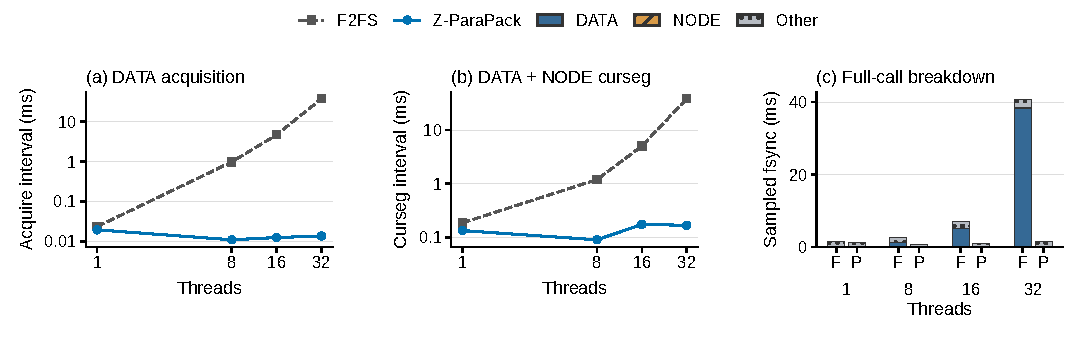
\includegraphics[width=\textwidth]{./figures/compact_fsync_breakdown.pdf}
\caption{Allocation intervals and full sampled fsync calls. (a) DATA curseg acquisition; (b) combined DATA/NODE curseg time; (c) full-call breakdown, with F/P denoting F2FS/Z-ParaPack. Lines and bars show sample means within independent diagnostic runs. The first two panels use logarithmic millisecond axes.}\label{fig:breakdown}
\end{figure*}

At 32 threads, DATA curseg acquisition falls from F2FS's 37.785\,ms to Z-ParaPack's 13.544\,$\mu$s.
Combined DATA/NODE curseg time falls from 38.369 to 0.168\,ms, occupying 12.2\% of Z-ParaPack's full sampled call.
The full call takes 1.378\,ms, 96.6\% shorter than F2FS.
These changes accord with the separated append state in Sections~\ref{sec:overview} through~\ref{sec:lease} and address the shared entry points in Figure~\ref{fig:motivation}.

Diagnostics use separate runs.
Allocation counts in Figure~\ref{fig:motivation}(b) use 64\,KiB writes followed by \texttt{fsync}, one/two/four threads, 16\,GiB per thread, and 60-second runs.
Figures~\ref{fig:motivation}(c) and~\ref{fig:breakdown} use one/eight/sixteen/32 threads, 256\,MiB per thread, and 30-second runs, sampling every 64th \texttt{fsync} per inode.
Each condition has one run, and both diagnostic protocols start after prefill and synchronization.
Path sampling covers the complete \texttt{fsync} and partitions DATA/NODE curseg acquisition and hold time into disjoint intervals, giving \texttt{balance} priority and assigning remaining time to Other.
Acquisition includes execution, queuing, and scheduling.
Z-ParaPack correlates local and delegated allocation callbacks for each request and classifies them by logical DATA/NODE type.

\textbf{CPU cost per write and synchronization tail latency.}
Figure~\ref{fig:cpu} uses the same 600-second performance runs as Figure~\ref{fig:scaling}(a, b), covering all six systems and conditions.
fio mean \texttt{fsync} latency weights each worker by its call count; tail latency takes the maximum worker p99.
CPU cost per completed write accumulates busy time across all logical CPUs over the full fio invocation, including filesystem threads, startup, and teardown.

At 4\,KiB and 32 threads, Z-ParaPack uses 182.64\,$\mu$s/write and has a maximum worker \texttt{fsync} p99 of 1.352\,ms.
F2FS, the fastest throughput baseline under that condition, uses 423.56\,$\mu$s/write with a 7.045\,ms tail.
At 64\,KiB and 32 threads, Z-ParaPack uses 635.69\,$\mu$s/write with a 2.966\,ms tail, compared with 815.50\,$\mu$s/write and 6.390\,ms for XFS.
As concurrent completion increases, host CPU time per completed write and synchronization tail latency also decrease.

\begin{figure*}[t]\centering
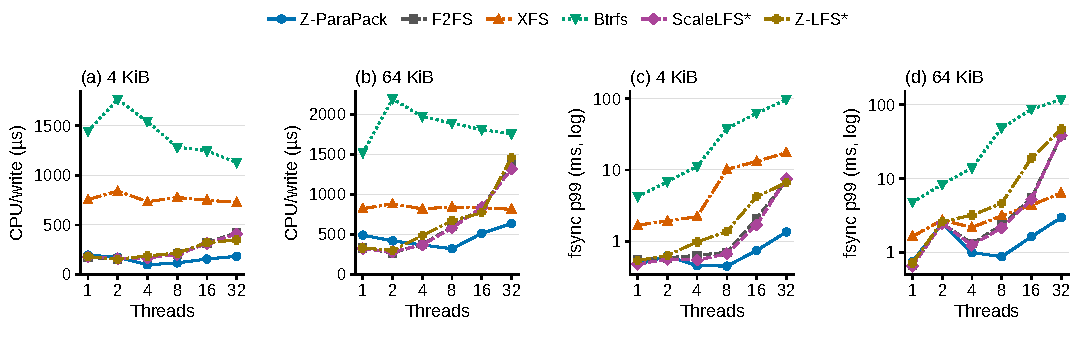
\includegraphics[width=\textwidth]{./figures/compact_fio_cost_tail.pdf}
\caption{Host CPU cost per completed write and maximum worker fsync p99. (a, b) CPU cost for 4\,KiB and 64\,KiB updates; (c, d) corresponding tail latency on logarithmic axes.}\label{fig:cpu}
\end{figure*}

\textbf{Namespace-commit reuse.}
The proof in Section~\ref{sec:namespace} lets subsequent synchronization reuse a completed checkpoint.
Enabling this mechanism within the same GOOD12.1 module increases throughput by 5.55\% and 5.00\% across two OceanBase controls.
It reduces p99 by 14.96\% and 13.41\%, respectively (Table~\ref{tab:namespace}).
These within-module controls use one instance, sixteen tenants, and four clients per tenant, totaling 64 clients.
Each state has one independent run under each order, OFF-to-ON and ON-to-OFF.
We analyze these separately from the 128-client cross-system comparison in Section~\ref{sec:applications}.
OceanBase merges transaction histograms within each run before computing tail latency.

\begin{table}[t]\centering
\caption{Within-module namespace-commit reuse with 64 clients.}\label{tab:namespace}
\small\setlength{\tabcolsep}{3pt}
\begin{tabular}{@{}llrr@{}}\toprule
Run order & State & Events/s & p99 (ms) \\
\midrule
OFF to ON & OFF & 11,031.04 & 23.521 \\
OFF to ON & ON & 11,642.76 & 20.002 \\
ON to OFF & OFF & 11,102.28 & 22.284 \\
ON to OFF & ON & 11,657.33 & 19.295 \\
\bottomrule\end{tabular}
\end{table}

The ON state reuses parent-number and directory-synchronization proofs; corresponding reuse counts remain zero in the OFF state.

\subsection{Commit Contents and Logical Recovery}\label{sec:logical}
Confirmed PACK contents remain recoverable after interruptions of subsequent commits.
Table~\ref{tab:recovery} organizes logical interruption scenarios around mapping closures, completion boundaries, and generation-scoped recovery in Sections~\ref{sec:closure}, \ref{sec:terminal}, and~\ref{sec:recovery}.
Z-ParaPack recovers complete files after successful \texttt{fsync} ACKs and continues with next-generation writes after restoring checkpoint state.
Experiments use the same GOOD12.1 module and Linux 7.2.9 virtual machines with memory-backed devices.
Predetermined complete file bytes provide the content oracle.
NOSYNC denotes interruption without generating a new checkpoint.

\begin{table}[t]\centering
\caption{GOOD12.1 content and logical recovery tests.}\label{tab:recovery}
\small\setlength{\tabcolsep}{3pt}
\begin{tabularx}{\columnwidth}{@{}P{.25\columnwidth}Y@{}}\toprule
Test group & Interruption scenario and content check \\
\midrule
Confirmed commits & Eight ACKs; recover after NOSYNC logical interruption and check all 32\,MiB byte for byte. \\
Incomplete terminal & Eight previous ACKs; inject a timeout before terminal submission, causing fsync to return EIO; interrupt the partial commit and recover the confirmed 32\,MiB. \\
Asynchronous mappings & Write DATA asynchronously, then synchronize pending mappings; eight ACKs; recover and check 32\,MiB after NOSYNC interruption. \\
Checkpoint and subsequent writes & Sixteen 192\,KiB files; checkpoint, then NOSYNC interruption; recover all bytes, write the next generation, and remount read-only; reclaim a checkpointed open-but-unlinked inode. \\
\bottomrule\end{tabularx}
\end{table}

The terminal distinguishes completed updates from partial commits.
All 32\,MiB confirmed by eight ACKs recover byte for byte after interruption.
Injecting a timeout before a subsequent terminal submission causes \texttt{fsync} to return EIO without damaging earlier acknowledged contents.
The asynchronous-writeback scenario first writes DATA, then synchronizes pending mappings, and recovers all 32\,MiB.
This tests the cross-lease obligation in Section~\ref{sec:joint}: mappings still require confirmation after DATA dirty flags clear.

Checkpoint recovery retains committed state and permits subsequent updates.
All sixteen 192\,KiB files match after recovery; read-only remount verifies next-generation writes, and recovery reclaims the checkpointed open-but-unlinked inode.
Across all four groups, both checkpoint packs retain identical complete bytes throughout the interruption window.
Post-remount checks inspect structure without repair.
Table~\ref{tab:recovery} tests logical interruptions on memory-backed devices and excludes physical power cuts.
Real-SSD performance runs use normal unmount/remount and content verification.
